\section{Smart Contract Idea and Evolution}

Smart contracts represent a milestone in the evolution of blockchain technology. They are electronic transaction protocols that execute the terms of a contract automatically and securely. Contrary to the perception of the term "\textit{smart}", smart contracts do not refer to contracts with artificial intelligence, but rather \textbf{executable programs} based on computer code.

As stated by \textbf{Nick Szabo} \cite{Szabo_1997}, the conceptual pioneer of this innovation:
\begin{quote}
{\Large\textbf{\textcolor{Orange}{“}}}A smart contract is an electronic transaction protocol that executes the terms of a contract. The general objectives are to satisfy common contractual conditions (such as payment terms, liens, confidentiality, and even enforcement), minimize exceptions both malicious and accidental, and minimize the need for trusted intermediaries. Related economic goals include lowering fraud loss, arbitrations and enforcement costs, and other transaction costs.{\Large\textbf{\textcolor{Orange}{”}}} 
\end{quote}
So, in essence, smart contracts promise to make contract processes more efficient, secure, and less burdensome by offering an innovative way to \textbf{automate and ensure the enforcement of contract terms}.

As with blockchain, smart contracts represent a combination of technologies that humans have created in their history. Below is a nice timeline (We hope the font will not make you ask, "\textit{Who lives in a pineapple under the sea?}"\img{tikz/chapter4 - Sponge.png}):

\vspace{-0.5cm}
\begin{figure}[!htbp]
\centering
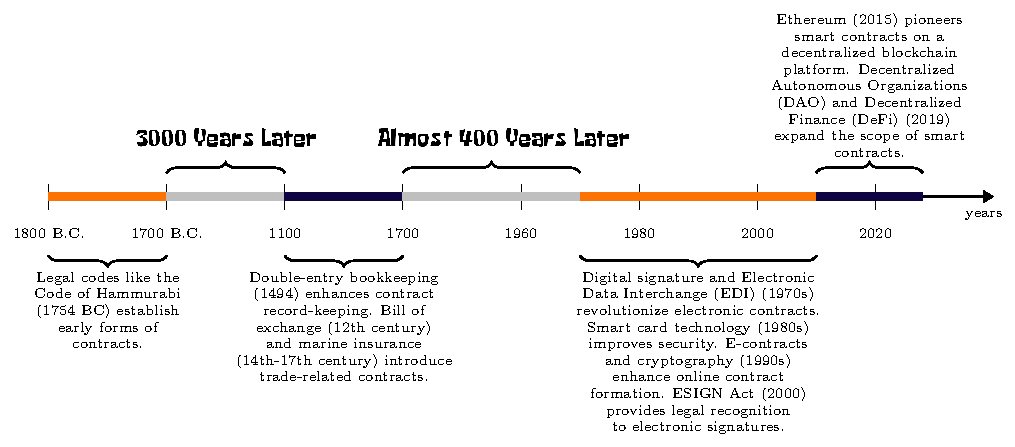
\includegraphics[width=\linewidth]{tikz/chapter4 - Smart Contract Timeline.pdf}
\caption{Smart Contracts Key Inventions Timeline}
\end{figure}


So what is different from a normal contract? In traditional contracts, the verbal text on paper is interpreted by human beings or lawyers ("wet" code). Their legal enforceability is subject to the \textbf{discretionary compliance and semantic flexibility} of human contracts. So, legal validity depends on the willingness of the parties involved to abide by the rules and the ability to interpret the text flexibly and adaptable to the situation.
On the other hand, smart contracts are rules and contracts executed as in a distribution machine ("dry" code). They are legally binding in a technological way, being contracts executed inexorably by code (as \textbf{Lessig} argues: "\textit{code is law}" \cite{les99}), which \textbf{cannot be violated and proceed unstoppably even if conditions have changed}.

\section{Ricardian Contracts}
A Ricardian contract is a legal document that is \textbf{comprehensible and accepted by both humans and machines}, and that is linked to all anticipated future operations (transactions). This type of contract possesses several distinctive properties. First, it is offered by an issuer to holders and represents a right of value managed by the issuer. It is easily readable by people, like a contract on paper, but is also interpretable by programmes, like a database. The contract is digitally signed and contains keys and server information, as well as being associated with a unique and secure identifier. This is basically an \textbf{evolution of the original contract}, indeed each contract can be represented by a graph of objects in prose, interacting in an ecosystem.

\textit{But hey, to really paint the picture, what sets it apart from a smart contract?} Ricardian Contracts focus primarily on being a primary document for the issuance of a digital asset, with an emphasis on \textbf{richer semantics}. In contrast, Smart Contracts are \textbf{more oriented towards programmability} and follow a deterministic approach. So, while Ricardians aim to provide a comprehensive document that is easily understood by all parties involved, Smart Contracts put more emphasis on automating contractual activities through code.

\textit{Let's put it in terms of desserts: Ricardian contracts are like grandma's homemade apple pie - wholesome, comforting, and always a crowd-pleaser. Smart contracts, on the other hand, are more like molecular gastronomy - innovative, impressive, but you're not entirely sure if it's still food...}

\section{Bitcoin or Ethereum? \texorpdfstring{\faBitcoin}{} \ \texorpdfstring{\faEthereum}{}}

Ethereum and Bitcoin differ significantly in their ability to execute smart contracts. \textbf{\textcolor{Orange}{Bitcoin}}, using a full non-Turing script language, is \textbf{limited in its ability to handle complex contracts} or sophisticated decentralised applications. On the other hand, \textbf{\textcolor{Orange}{Ethereum}} offers a \textbf{more powerful environment for smart contracts} through the Solidity language, running on its \textbf{Ethereum virtual machines} (EVMs), which are full Turing. This allows developers to create much more sophisticated smart contracts on Ethereum, with the ability to perform a wide range of calculations or programmable logic. In short, Ethereum offers a more flexible and powerful platform for smart contract development than Bitcoin.

\section{Smart Contract Compliance Issues}
There are several problems with smart contracts that can cause uncertainty and legal challenges:
\begin{enumerate}
    \item \textbf{\textcolor{Blue}{Understanding the Computer Code}}: courts and parties involved may have difficulty understanding the computer code on which smart contracts are based. This can make it difficult to assess all contractual obligations and terms fully and accurately.
    \item \textbf{\textcolor{Blue}{Legal Bindingness}}: in some jurisdictions, the legality and bindingness of smart contracts are not clearly defined. Some courts may not recognise smart contracts as legally binding agreements.
    \item \textbf{\textcolor{Blue}{Determinism of Smart Contracts}}: smart contracts operate deterministically, performing only what they have been programmed to do. This means that they cannot adapt or resolve situations not foreseen in the code.
    \item \textbf{\textcolor{Blue}{Legal Considerations and Exceptions}}: there are many legal considerations and exceptions that must be taken into account when entering into a contract. Smart contracts may not be able to handle these complex situations effectively.
    \item \textbf{\textcolor{Blue}{Different Laws and Jurisdictions}}: laws and jurisdictions vary from country to country. Some jurisdictions may be more favourable to the recognition of smart contracts than others.
\end{enumerate}
Taken together, these factors contribute to smart contracts being subject to legal uncertainty and may require further regulation and clarification to be fully accepted and reliably used.

\textbf{\textcolor{Orange}{Smart Legal Contracts}} are an evolution of traditional smart contracts, offering a solution to address the legal challenges associated with their implementation. While smart contracts consist of computer code and operate according to the "code is law" principle, Smart Legal Contracts combine legal language, parameters and code to create a legally binding contract.

The main objective of Smart Legal Contracts is to provide neutral performance within the terms and conditions defined by the contractual parties. Unlike smart contracts, Smart Legal Contracts recognise that the \textbf{law has the final word and may be subject to legal interpretation and modification}.

In terms of modifiability, Smart Legal Contracts offer \textbf{more flexibility than traditional smart contracts}. While the code of smart contracts cannot be changed once activated, Smart Legal Contracts allow changes to the code and can be paused if necessary.

That's why Smart Legal Contracts find application in a \textbf{wide range of industries and types of agreements}, as they offer a solution for creating legally binding contracts that also incorporate code-based automation and execution elements.

\section{DApps}

Now that we have studied smart contracts in detail, it is time to turn our gaze towards the stars of the show: the DApps. However, before we let ourselves be enchanted by their wonders, it is crucial to take a closer look at the ecosystem that supports them. This overview not only prepares us for the next act, but also shows us the interconnection and synergy between the layers that make the DApp venture possible. 

\begin{figure}[!htbp]
\centering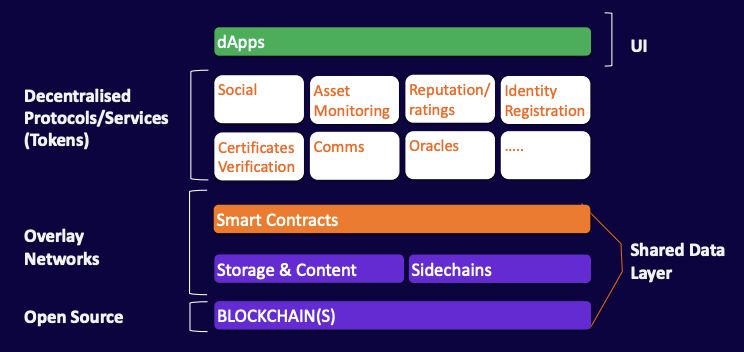
\includegraphics[scale=0.75]{tikz/chapter4 - Blockchain Stack.png}
\caption{Representation of the Blockchain Stack}
\end{figure}

From bottom to top:
\begin{itemize}
    \item \textbf{Blockchain}: This is the foundation on which the entire ecosystem is based. 
    \item \textbf{Storage, Content and Sidechains}: This layer manages the storage of data and the content associated with transactions on the blockchain. It also includes sidechains, which are separate blockchains connected to the main blockchain. Sidechains allow specific transactions to be performed without clogging up the main blockchain, improving scalability and enabling experimentation with new functionality without compromising security.
    \item \textbf{Smart Contracts}: \textit{We have just seen them :)}
    \item \textbf{Decentralised Protocols and Services}: This layer comprises the decentralised protocols and services that enable the creation, management and exchange of digital tokens on the blockchain. \textbf{Tokens} can represent digital currency, digital assets, rights to use resources and much more. These protocols and services provide a standardised infrastructure to facilitate the interoperability and adoption of tokens within the blockchain ecosystem.
    \item \textbf{DApps}: This is the highest layer of the stack and represents decentralised applications that utilise the layers below to provide a wide range of services and functionality to users. DApps exploit the unique features of blockchain, such as security, immunity from censorship and transparency, to offer innovative and reliable solutions.
\end{itemize}

Basically, decentralised applications are software programmes that operate by different methods. In addition to their underlying architecture and functionality, DApps may also present different \textbf{user interfaces} (UIs) to allow users to interact with them in intuitive and user-friendly ways. They are generally classified into three types: Type 1, Type 2 or Type 3.

\begin{table}[h]
\begin{tabularx}{\linewidth}{>{\parskip1ex}X@{\kern2\tabcolsep}>{\parskip1ex}X@{\kern2\tabcolsep}>{\parskip1ex}X}
\toprule
\hfil\bfseries \color{Orange}{Type 1}
&
\hfil\bfseries \color{Orange}{Type 2}
&
\hfil\bfseries \color{Orange}{Type 3}
\\\cmidrule(r{-\tabcolsep}){1-1}\cmidrule(lr{-\tabcolsep}){2-2}\cmidrule(l{-\tabcolsep}){3-3}

%% TYPE 1
Type 1 DApps operate on their own \textbf{\color{Blue}{dedicated blockchain}}. A prominent example of this is Ethereum-based smart contract DApps. These DApps, such as decentralized finance (DeFi) applications, execute on the Ethereum blockchain and may utilize a native token like ETH.
&
%% TYPE 2
Type 2 DApps utilize an \textbf{\color{Blue}{existing established blockchain}}. They rely on Type 1 blockchains and introduce custom protocols and tokens. For instance, DAI is built on top of Ethereum but features its own stablecoins and mechanisms for distribution and governance.
&
%% TYPE 3
Type 3 DApps leverage the \textbf{\color{Blue}{protocols of Type 2 DApps}}. An example is the SAFE Network, which utilizes the OMNI network protocol. These DApps build upon existing decentralized infrastructure to offer specialized functionalities.
\\
\bottomrule
\end{tabularx}
\caption{Benefits, Limitations, and Additional Considerations of Blockchain Technology}
\end{table}

DApps must be completely open source and autonomous, with no one entity controlling most of their tokens, changes must be based on community consensus, data must be cryptographically secure on a decentralised public blockchain, and a cryptographic token must be used for access and to incentivise contributors, generated by the DApp itself as proof of value.

\section{Oracles}
Unfortunately, smart contracts, and consequently DApps, do not have the ability to directly access external data. However, to overcome this limitation, special tools called \textbf{oracles} come into play. 

In DApps, oracles act as a bridge between the real world and the blockchain, allowing smart contracts to \textbf{access external data} and perform actions in response to certain conditions. Oracles are services provided by third parties and are designed to provide reliable external data to smart contracts on the blockchain. This data can cover a wide range of information, such as weather conditions, payment confirmations or price changes.

The operation of oracles varies depending on the implementation and the blockchain used. In Bitcoin, for example, an oracle can write \textbf{data about a specific transaction}, while in Ethereum, data can be \textbf{stored in the smart contract} itself for use by other smart contracts through message calls.

Oracles are key to enabling DApps to interact with the outside world and perform actions based on real events, thus expanding the possibilities of blockchain usage beyond the confines of the closed system of the blockchain itself.

\section{Blockchain and Smart Contracts Summary}
Here we include schemes that summarise the various concepts we have addressed in these sections:
\begin{figure}[!htbp]
\centering
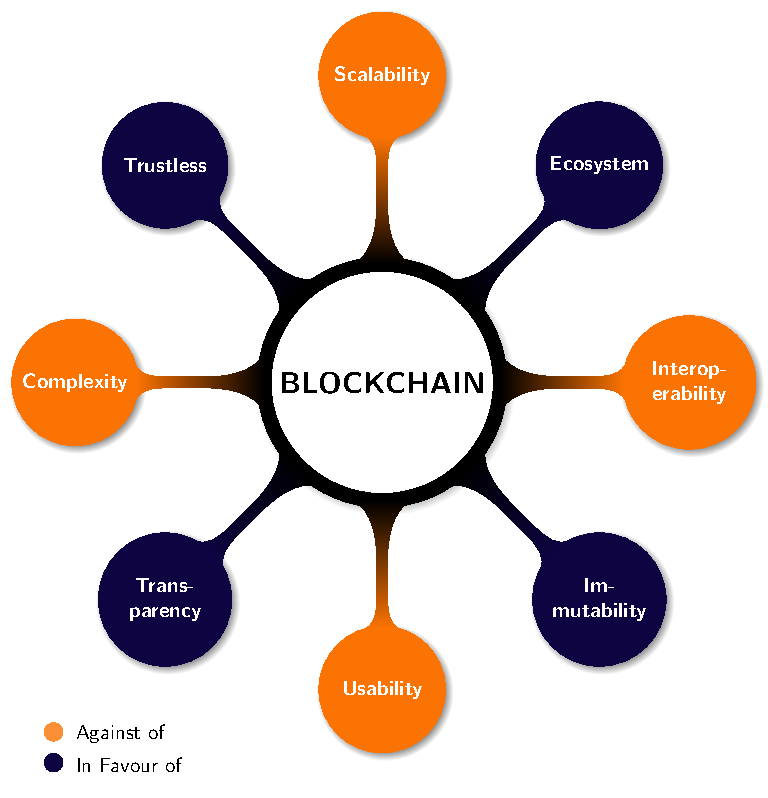
\includegraphics[width=0.7\linewidth]{tikz/chapter4 - Blockchain Summary.pdf}
\caption{Blockchain Concepts Summary}
\end{figure}

\

\begin{figure}[!htbp]
\centering
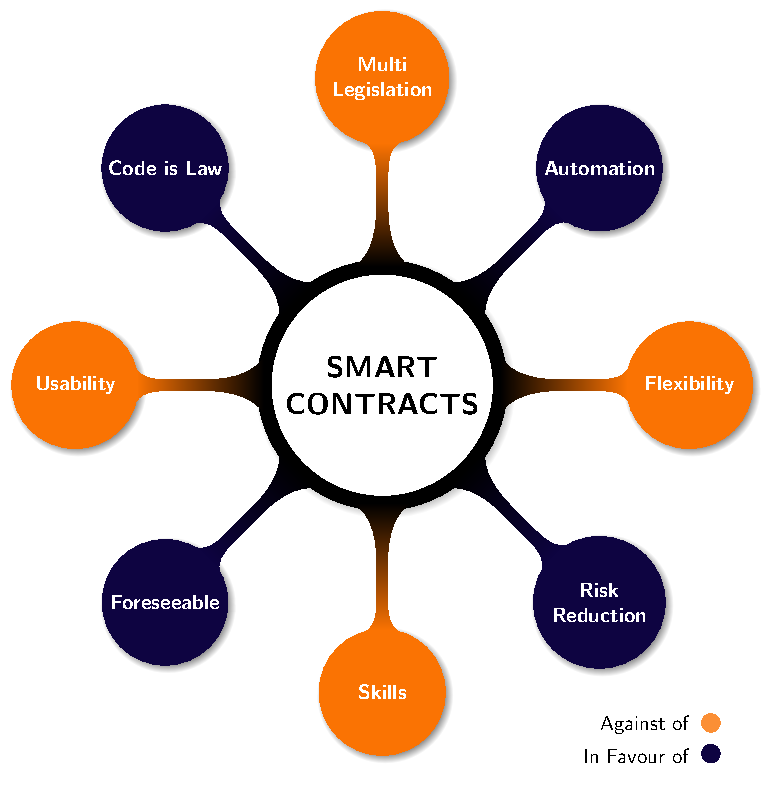
\includegraphics[width=0.7\linewidth]{tikz/chapter4 - Smart Contracts Summary.pdf}
\caption{Smart Contracts Concepts Summary}
\end{figure}